\documentclass[1p]{elsarticle_modified}
%\bibliographystyle{elsarticle-num}

%\usepackage[colorlinks]{hyperref}
%\usepackage{abbrmath_seonhwa} %\Abb, \Ascr, \Acal ,\Abf, \Afrak
\usepackage{amsfonts}
\usepackage{amssymb}
\usepackage{amsmath}
\usepackage{amsthm}
\usepackage{scalefnt}
\usepackage{amsbsy}
\usepackage{kotex}
\usepackage{caption}
\usepackage{subfig}
\usepackage{color}
\usepackage{graphicx}
\usepackage{xcolor} %% white, black, red, green, blue, cyan, magenta, yellow
\usepackage{float}
\usepackage{setspace}
\usepackage{hyperref}

\usepackage{tikz}
\usetikzlibrary{arrows}

\usepackage{multirow}
\usepackage{array} % fixed length table
\usepackage{hhline}

%%%%%%%%%%%%%%%%%%%%%
\makeatletter
\renewcommand*\env@matrix[1][\arraystretch]{%
	\edef\arraystretch{#1}%
	\hskip -\arraycolsep
	\let\@ifnextchar\new@ifnextchar
	\array{*\c@MaxMatrixCols c}}
\makeatother %https://tex.stackexchange.com/questions/14071/how-can-i-increase-the-line-spacing-in-a-matrix
%%%%%%%%%%%%%%%

\usepackage[normalem]{ulem}

\newcommand{\msout}[1]{\ifmmode\text{\sout{\ensuremath{#1}}}\else\sout{#1}\fi}
%SOURCE: \msout is \stkout macro in https://tex.stackexchange.com/questions/20609/strikeout-in-math-mode

\newcommand{\cancel}[1]{
	\ifmmode
	{\color{red}\msout{#1}}
	\else
	{\color{red}\sout{#1}}
	\fi
}

\newcommand{\add}[1]{
	{\color{blue}\uwave{#1}}
}

\newcommand{\replace}[2]{
	\ifmmode
	{\color{red}\msout{#1}}{\color{blue}\uwave{#2}}
	\else
	{\color{red}\sout{#1}}{\color{blue}\uwave{#2}}
	\fi
}

\newcommand{\Sol}{\mathcal{S}} %segment
\newcommand{\D}{D} %diagram
\newcommand{\A}{\mathcal{A}} %arc


%%%%%%%%%%%%%%%%%%%%%%%%%%%%%5 test

\def\sl{\operatorname{\textup{SL}}(2,\Cbb)}
\def\psl{\operatorname{\textup{PSL}}(2,\Cbb)}
\def\quan{\mkern 1mu \triangleright \mkern 1mu}

\theoremstyle{definition}
\newtheorem{thm}{Theorem}[section]
\newtheorem{prop}[thm]{Proposition}
\newtheorem{lem}[thm]{Lemma}
\newtheorem{ques}[thm]{Question}
\newtheorem{cor}[thm]{Corollary}
\newtheorem{defn}[thm]{Definition}
\newtheorem{exam}[thm]{Example}
\newtheorem{rmk}[thm]{Remark}
\newtheorem{alg}[thm]{Algorithm}

\newcommand{\I}{\sqrt{-1}}
\begin{document}

%\begin{frontmatter}
%
%\title{Boundary parabolic representations of knots up to 8 crossings}
%
%%% Group authors per affiliation:
%\author{Yunhi Cho} 
%\address{Department of Mathematics, University of Seoul, Seoul, Korea}
%\ead{yhcho@uos.ac.kr}
%
%
%\author{Seonhwa Kim} %\fnref{s_kim}}
%\address{Center for Geometry and Physics, Institute for Basic Science, Pohang, 37673, Korea}
%\ead{ryeona17@ibs.re.kr}
%
%\author{Hyuk Kim}
%\address{Department of Mathematical Sciences, Seoul National University, Seoul 08826, Korea}
%\ead{hyukkim@snu.ac.kr}
%
%\author{Seokbeom Yoon}
%\address{Department of Mathematical Sciences, Seoul National University, Seoul, 08826,  Korea}
%\ead{sbyoon15@snu.ac.kr}
%
%\begin{abstract}
%We find all boundary parabolic representation of knots up to 8 crossings.
%
%\end{abstract}
%\begin{keyword}
%    \MSC[2010] 57M25 
%\end{keyword}
%
%\end{frontmatter}

%\linenumbers
%\tableofcontents
%
\newcommand\colored[1]{\textcolor{white}{\rule[-0.35ex]{0.8em}{1.4ex}}\kern-0.8em\color{red} #1}%
%\newcommand\colored[1]{\textcolor{white}{ #1}\kern-2.17ex	\textcolor{white}{ #1}\kern-1.81ex	\textcolor{white}{ #1}\kern-2.15ex\color{red}#1	}

{\Large $\underline{12a_{0188}~(K12a_{0188})}$}

\setlength{\tabcolsep}{10pt}
\renewcommand{\arraystretch}{1.6}
\vspace{1cm}\begin{tabular}{m{100pt}>{\centering\arraybackslash}m{274pt}}
\multirow{5}{120pt}{
	\centering
	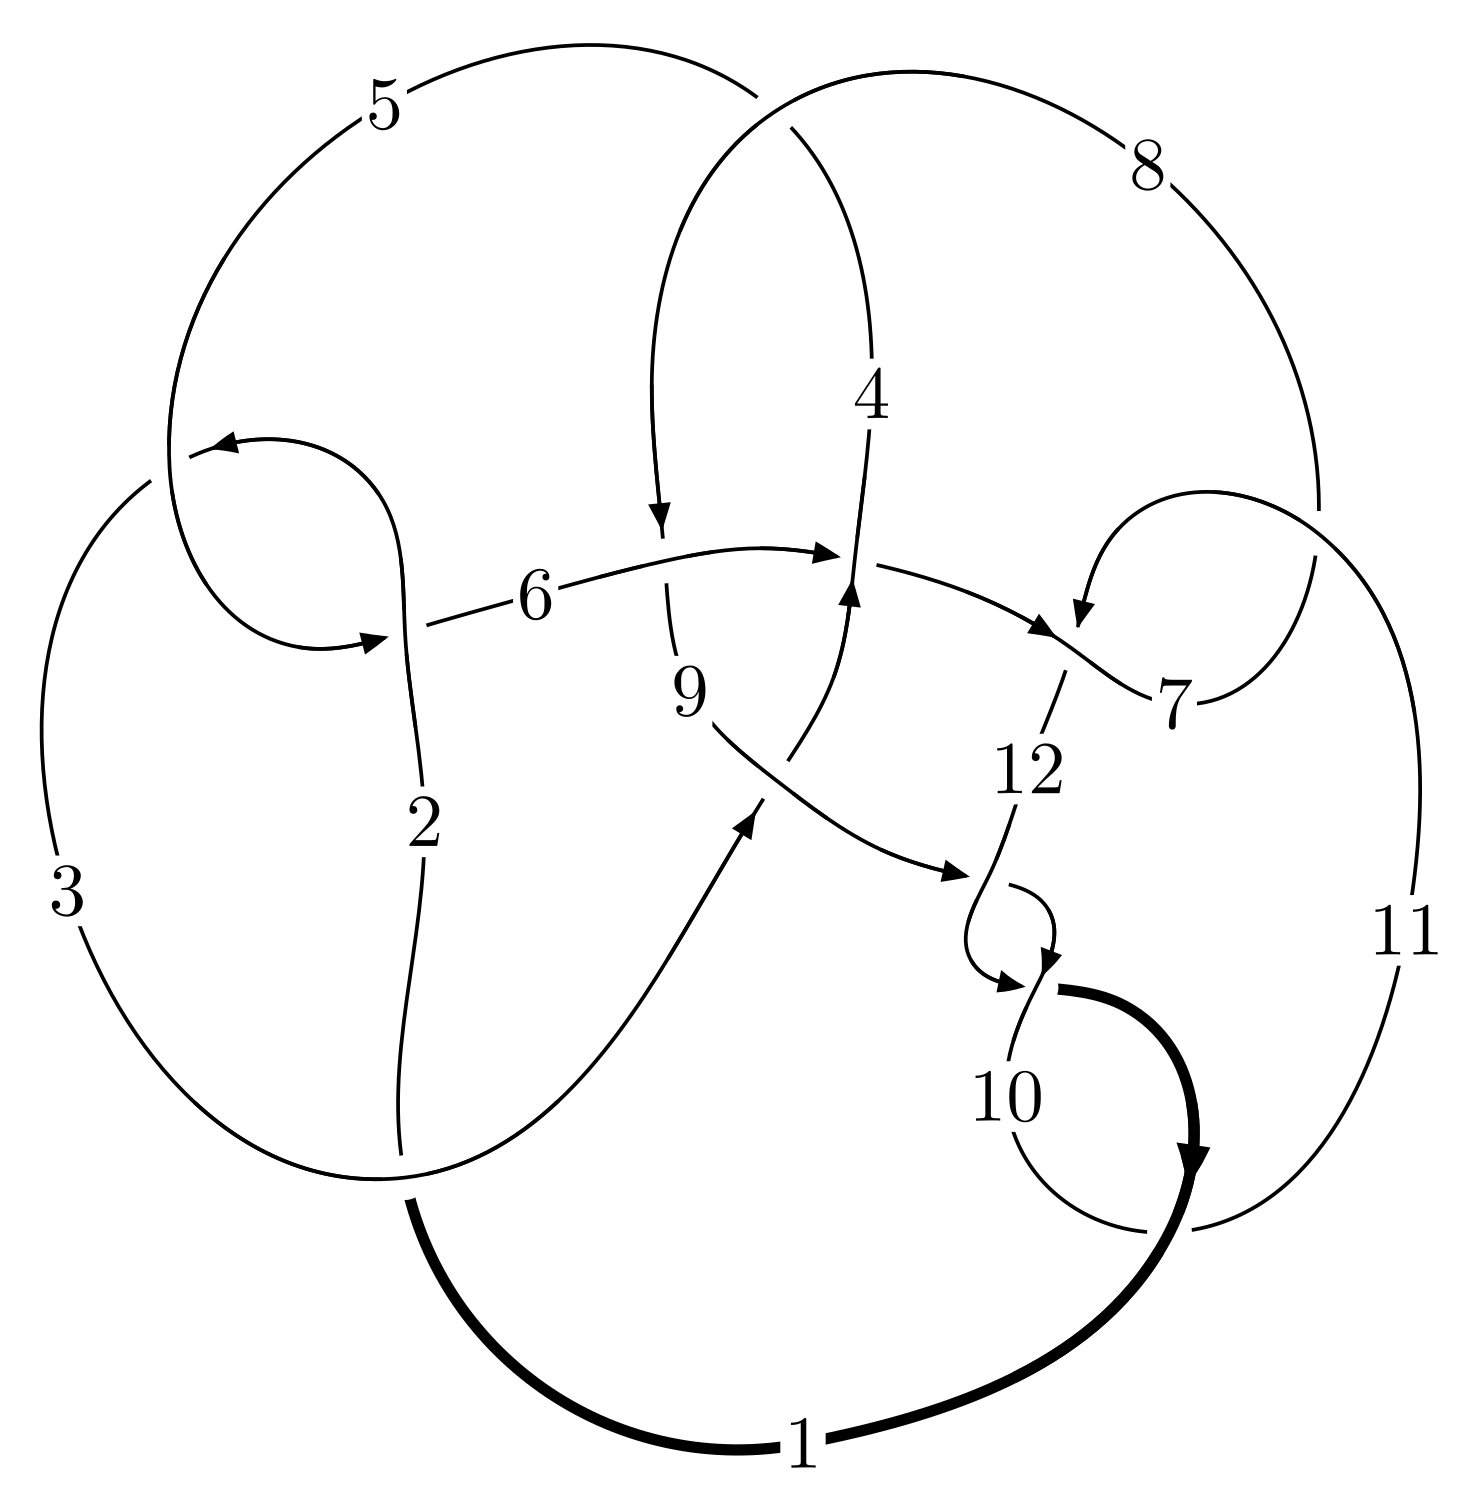
\includegraphics[width=112pt]{../../../GIT/diagram.site/Diagrams/png/989_12a_0188.png}\\
\ \ \ A knot diagram\footnotemark}&
\allowdisplaybreaks
\textbf{Linearized knot diagam} \\
\cline{2-2}
 &
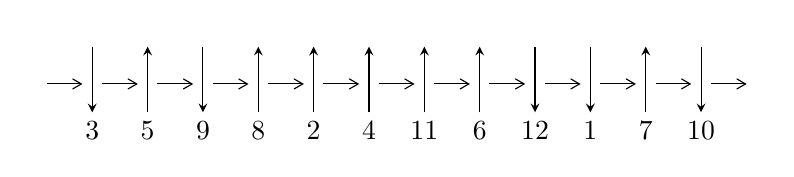
\begin{tikzpicture}[x=20pt, y=17pt]
	% nodes
	\node (C0) at (0, 0) {};
	\node (C1) at (1, 0) {};
	\node (C1U) at (1, +1) {};
	\node (C1D) at (1, -1) {3};

	\node (C2) at (2, 0) {};
	\node (C2U) at (2, +1) {};
	\node (C2D) at (2, -1) {5};

	\node (C3) at (3, 0) {};
	\node (C3U) at (3, +1) {};
	\node (C3D) at (3, -1) {9};

	\node (C4) at (4, 0) {};
	\node (C4U) at (4, +1) {};
	\node (C4D) at (4, -1) {8};

	\node (C5) at (5, 0) {};
	\node (C5U) at (5, +1) {};
	\node (C5D) at (5, -1) {2};

	\node (C6) at (6, 0) {};
	\node (C6U) at (6, +1) {};
	\node (C6D) at (6, -1) {4};

	\node (C7) at (7, 0) {};
	\node (C7U) at (7, +1) {};
	\node (C7D) at (7, -1) {11};

	\node (C8) at (8, 0) {};
	\node (C8U) at (8, +1) {};
	\node (C8D) at (8, -1) {6};

	\node (C9) at (9, 0) {};
	\node (C9U) at (9, +1) {};
	\node (C9D) at (9, -1) {12};

	\node (C10) at (10, 0) {};
	\node (C10U) at (10, +1) {};
	\node (C10D) at (10, -1) {1};

	\node (C11) at (11, 0) {};
	\node (C11U) at (11, +1) {};
	\node (C11D) at (11, -1) {7};

	\node (C12) at (12, 0) {};
	\node (C12U) at (12, +1) {};
	\node (C12D) at (12, -1) {10};
	\node (C13) at (13, 0) {};

	% arrows
	\draw[->,>={angle 60}]
	(C0) edge (C1) (C1) edge (C2) (C2) edge (C3) (C3) edge (C4) (C4) edge (C5) (C5) edge (C6) (C6) edge (C7) (C7) edge (C8) (C8) edge (C9) (C9) edge (C10) (C10) edge (C11) (C11) edge (C12) (C12) edge (C13) ;	\draw[->,>=stealth]
	(C1U) edge (C1D) (C2D) edge (C2U) (C3U) edge (C3D) (C4D) edge (C4U) (C5D) edge (C5U) (C6D) edge (C6U) (C7D) edge (C7U) (C8D) edge (C8U) (C9U) edge (C9D) (C10U) edge (C10D) (C11D) edge (C11U) (C12U) edge (C12D) ;
	\end{tikzpicture} \\
\hhline{~~} \\& 
\textbf{Solving Sequence} \\ \cline{2-2} 
 &
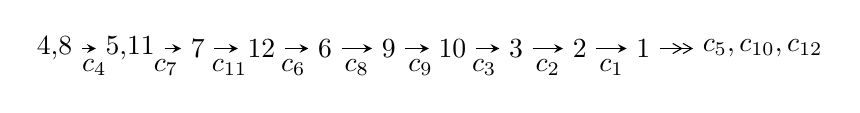
\begin{tikzpicture}[x=23pt, y=7pt]
	% node
	\node (A0) at (-1/8, 0) {4,8};
	\node (A1) at (17/16, 0) {5,11};
	\node (A2) at (17/8, 0) {7};
	\node (A3) at (25/8, 0) {12};
	\node (A4) at (33/8, 0) {6};
	\node (A5) at (41/8, 0) {9};
	\node (A6) at (49/8, 0) {10};
	\node (A7) at (57/8, 0) {3};
	\node (A8) at (65/8, 0) {2};
	\node (A9) at (73/8, 0) {1};
	\node (C1) at (1/2, -1) {$c_{4}$};
	\node (C2) at (13/8, -1) {$c_{7}$};
	\node (C3) at (21/8, -1) {$c_{11}$};
	\node (C4) at (29/8, -1) {$c_{6}$};
	\node (C5) at (37/8, -1) {$c_{8}$};
	\node (C6) at (45/8, -1) {$c_{9}$};
	\node (C7) at (53/8, -1) {$c_{3}$};
	\node (C8) at (61/8, -1) {$c_{2}$};
	\node (C9) at (69/8, -1) {$c_{1}$};
	\node (A10) at (11, 0) {$c_{5},c_{10},c_{12}$};

	% edge
	\draw[->,>=stealth]	
	(A0) edge (A1) (A1) edge (A2) (A2) edge (A3) (A3) edge (A4) (A4) edge (A5) (A5) edge (A6) (A6) edge (A7) (A7) edge (A8) (A8) edge (A9) ;
	\draw[->>,>={angle 60}]	
	(A9) edge (A10);
\end{tikzpicture} \\ 

\end{tabular} \\

\footnotetext{
The image of knot diagram is generated by the software ``\textbf{Draw programme}" developed by Andrew Bartholomew(\url{http://www.layer8.co.uk/maths/draw/index.htm\#Running-draw}), where we modified some parts for our purpose(\url{https://github.com/CATsTAILs/LinksPainter}).
}\phantom \\ \newline 
\centering \textbf{Ideals for irreducible components\footnotemark of $X_{\text{par}}$} 
 
\begin{align*}
I^u_{1}&=\langle 
-7.42605\times10^{1018} u^{118}-1.10416\times10^{1019} u^{117}+\cdots+2.49080\times10^{1022} b-2.03299\times10^{1022},\\
\phantom{I^u_{1}}&\phantom{= \langle  }3.47903\times10^{1021} u^{118}+6.79805\times10^{1021} u^{117}+\cdots+6.61059\times10^{1024} a-1.30130\times10^{1025},\\
\phantom{I^u_{1}}&\phantom{= \langle  }u^{119}+2 u^{118}+\cdots+8762 u+1327\rangle \\
I^u_{2}&=\langle 
u^8-2 u^6+2 u^4+u^3+b- u+1,\;a,\;u^9- u^8-2 u^7+3 u^6+u^5-3 u^4+2 u^3- u+1\rangle \\
\\
\end{align*}
\raggedright * 2 irreducible components of $\dim_{\mathbb{C}}=0$, with total 128 representations.\\
\footnotetext{All coefficients of polynomials are rational numbers. But the coefficients are sometimes approximated in decimal forms when there is not enough margin.}
\newpage
\renewcommand{\arraystretch}{1}
\centering \section*{I. $I^u_{1}= \langle -7.43\times10^{1018} u^{118}-1.10\times10^{1019} u^{117}+\cdots+2.49\times10^{1022} b-2.03\times10^{1022},\;3.48\times10^{1021} u^{118}+6.80\times10^{1021} u^{117}+\cdots+6.61\times10^{1024} a-1.30\times10^{1025},\;u^{119}+2 u^{118}+\cdots+8762 u+1327 \rangle$}
\flushleft \textbf{(i) Arc colorings}\\
\begin{tabular}{m{7pt} m{180pt} m{7pt} m{180pt} }
\flushright $a_{4}=$&$\begin{pmatrix}1\\0\end{pmatrix}$ \\
\flushright $a_{8}=$&$\begin{pmatrix}0\\u\end{pmatrix}$ \\
\flushright $a_{5}=$&$\begin{pmatrix}1\\- u^2\end{pmatrix}$ \\
\flushright $a_{11}=$&$\begin{pmatrix}-0.000526281 u^{118}-0.00102836 u^{117}+\cdots-12.9920 u+1.96851\\0.000298139 u^{118}+0.000443295 u^{117}+\cdots+2.48668 u+0.816199\end{pmatrix}$ \\
\flushright $a_{7}=$&$\begin{pmatrix}-0.00204675 u^{118}-0.00374735 u^{117}+\cdots-44.8125 u-10.1681\\0.000217932 u^{118}+0.000446866 u^{117}+\cdots+2.65443 u+1.01512\end{pmatrix}$ \\
\flushright $a_{12}=$&$\begin{pmatrix}-0.00340766 u^{118}-0.00621070 u^{117}+\cdots-43.0873 u-17.5112\\-0.0000110966 u^{118}-0.0000853887 u^{117}+\cdots+0.224165 u+0.246586\end{pmatrix}$ \\
\flushright $a_{6}=$&$\begin{pmatrix}-0.00226468 u^{118}-0.00419422 u^{117}+\cdots-47.4669 u-11.1832\\0.000217932 u^{118}+0.000446866 u^{117}+\cdots+2.65443 u+1.01512\end{pmatrix}$ \\
\flushright $a_{9}=$&$\begin{pmatrix}0.000279013 u^{118}+0.000673242 u^{117}+\cdots-23.4449 u+9.53210\\0.000478417 u^{118}+0.000913280 u^{117}+\cdots+4.42620 u+2.18078\end{pmatrix}$ \\
\flushright $a_{10}=$&$\begin{pmatrix}0.000991558 u^{118}+0.00190829 u^{117}+\cdots+2.65205 u+5.62220\\0.000451996 u^{118}+0.000840247 u^{117}+\cdots+8.82580 u+1.76896\end{pmatrix}$ \\
\flushright $a_{3}=$&$\begin{pmatrix}-0.00208611 u^{118}-0.00412377 u^{117}+\cdots-34.1619 u-20.6382\\-0.000442936 u^{118}-0.000823798 u^{117}+\cdots-10.8522 u-2.78052\end{pmatrix}$ \\
\flushright $a_{2}=$&$\begin{pmatrix}-0.00157316 u^{118}-0.00308242 u^{117}+\cdots-25.6536 u-17.7935\\-0.000473190 u^{118}-0.000917918 u^{117}+\cdots-10.0361 u-2.76001\end{pmatrix}$ \\
\flushright $a_{1}=$&$\begin{pmatrix}-0.00406489 u^{118}-0.00755589 u^{117}+\cdots-73.4388 u-20.9068\\-0.000730125 u^{118}-0.00137620 u^{117}+\cdots-12.0660 u-1.83313\end{pmatrix}$\\&\end{tabular}
\flushleft \textbf{(ii) Obstruction class $= -1$}\\~\\
\flushleft \textbf{(iii) Cusp Shapes $= 0.00267969 u^{118}+0.00463437 u^{117}+\cdots+47.3827 u+19.3117$}\\~\\
\newpage\renewcommand{\arraystretch}{1}
\flushleft \textbf{(iv) u-Polynomials at the component}\newline \\
\begin{tabular}{m{50pt}|m{274pt}}
Crossings & \hspace{64pt}u-Polynomials at each crossing \\
\hline $$\begin{aligned}c_{1}\end{aligned}$$&$\begin{aligned}
&u^{119}+48 u^{118}+\cdots-10 u-1
\end{aligned}$\\
\hline $$\begin{aligned}c_{2},c_{5}\end{aligned}$$&$\begin{aligned}
&u^{119}+2 u^{118}+\cdots-10 u-1
\end{aligned}$\\
\hline $$\begin{aligned}c_{3}\end{aligned}$$&$\begin{aligned}
&u^{119}-6 u^{118}+\cdots-3844 u-1441
\end{aligned}$\\
\hline $$\begin{aligned}c_{4}\end{aligned}$$&$\begin{aligned}
&u^{119}-2 u^{118}+\cdots+8762 u-1327
\end{aligned}$\\
\hline $$\begin{aligned}c_{6}\end{aligned}$$&$\begin{aligned}
&u^{119}+12 u^{118}+\cdots-2 u-1
\end{aligned}$\\
\hline $$\begin{aligned}c_{7},c_{11}\end{aligned}$$&$\begin{aligned}
&u^{119}- u^{118}+\cdots+4096 u-512
\end{aligned}$\\
\hline $$\begin{aligned}c_{8}\end{aligned}$$&$\begin{aligned}
&u^{119}+10 u^{118}+\cdots-2 u-1
\end{aligned}$\\
\hline $$\begin{aligned}c_{9},c_{10},c_{12}\end{aligned}$$&$\begin{aligned}
&u^{119}-10 u^{118}+\cdots+14 u-1
\end{aligned}$\\
\hline
\end{tabular}\\~\\
\newpage\renewcommand{\arraystretch}{1}
\flushleft \textbf{(v) Riley Polynomials at the component}\newline \\
\begin{tabular}{m{50pt}|m{274pt}}
Crossings & \hspace{64pt}Riley Polynomials at each crossing \\
\hline $$\begin{aligned}c_{1}\end{aligned}$$&$\begin{aligned}
&y^{119}+48 y^{118}+\cdots-1922 y-1
\end{aligned}$\\
\hline $$\begin{aligned}c_{2},c_{5}\end{aligned}$$&$\begin{aligned}
&y^{119}+48 y^{118}+\cdots-10 y-1
\end{aligned}$\\
\hline $$\begin{aligned}c_{3}\end{aligned}$$&$\begin{aligned}
&y^{119}-108 y^{118}+\cdots-880963674 y-2076481
\end{aligned}$\\
\hline $$\begin{aligned}c_{4}\end{aligned}$$&$\begin{aligned}
&y^{119}-132 y^{118}+\cdots+73112778 y-1760929
\end{aligned}$\\
\hline $$\begin{aligned}c_{6}\end{aligned}$$&$\begin{aligned}
&y^{119}+100 y^{117}+\cdots-10 y-1
\end{aligned}$\\
\hline $$\begin{aligned}c_{7},c_{11}\end{aligned}$$&$\begin{aligned}
&y^{119}+57 y^{118}+\cdots-1572864 y-262144
\end{aligned}$\\
\hline $$\begin{aligned}c_{8}\end{aligned}$$&$\begin{aligned}
&y^{119}-12 y^{118}+\cdots+10 y-1
\end{aligned}$\\
\hline $$\begin{aligned}c_{9},c_{10},c_{12}\end{aligned}$$&$\begin{aligned}
&y^{119}-108 y^{118}+\cdots-162 y-1
\end{aligned}$\\
\hline
\end{tabular}\\~\\
\newpage\flushleft \textbf{(vi) Complex Volumes and Cusp Shapes}
$$\begin{array}{c|c|c}  
\text{Solutions to }I^u_{1}& \I (\text{vol} + \sqrt{-1}CS) & \text{Cusp shape}\\
 \hline 
\begin{aligned}
u &= -0.081525 + 0.998574 I \\
a &= -1.41965 + 0.28773 I \\
b &= -1.59460 - 0.55588 I\end{aligned}
 & -13.32730 + 0.47174 I & \phantom{-0.000000 } 0 \\ \hline\begin{aligned}
u &= -0.081525 - 0.998574 I \\
a &= -1.41965 - 0.28773 I \\
b &= -1.59460 + 0.55588 I\end{aligned}
 & -13.32730 - 0.47174 I & \phantom{-0.000000 } 0 \\ \hline\begin{aligned}
u &= -0.970650 + 0.184323 I \\
a &= \phantom{-}0.271720 + 1.164900 I \\
b &= \phantom{-}0.118861 + 0.924692 I\end{aligned}
 & -1.80179 + 3.47511 I & \phantom{-0.000000 } 0 \\ \hline\begin{aligned}
u &= -0.970650 - 0.184323 I \\
a &= \phantom{-}0.271720 - 1.164900 I \\
b &= \phantom{-}0.118861 - 0.924692 I\end{aligned}
 & -1.80179 - 3.47511 I & \phantom{-0.000000 } 0 \\ \hline\begin{aligned}
u &= -0.910650 + 0.368955 I \\
a &= \phantom{-}0.869458 + 0.182486 I \\
b &= \phantom{-}0.1018280 - 0.0457066 I\end{aligned}
 & \phantom{-}3.48096 - 0.06555 I & \phantom{-0.000000 } 0 \\ \hline\begin{aligned}
u &= -0.910650 - 0.368955 I \\
a &= \phantom{-}0.869458 - 0.182486 I \\
b &= \phantom{-}0.1018280 + 0.0457066 I\end{aligned}
 & \phantom{-}3.48096 + 0.06555 I & \phantom{-0.000000 } 0 \\ \hline\begin{aligned}
u &= \phantom{-}0.704399 + 0.664447 I \\
a &= \phantom{-}0.226012 - 0.547602 I \\
b &= -0.360213 - 0.109997 I\end{aligned}
 & -1.94863 + 2.48320 I & \phantom{-0.000000 } 0 \\ \hline\begin{aligned}
u &= \phantom{-}0.704399 - 0.664447 I \\
a &= \phantom{-}0.226012 + 0.547602 I \\
b &= -0.360213 + 0.109997 I\end{aligned}
 & -1.94863 - 2.48320 I & \phantom{-0.000000 } 0 \\ \hline\begin{aligned}
u &= -0.433604 + 0.853701 I \\
a &= \phantom{-}1.036840 - 0.408640 I \\
b &= \phantom{-}1.89884 + 0.99868 I\end{aligned}
 & -5.55472 - 1.58319 I & \phantom{-0.000000 } 0 \\ \hline\begin{aligned}
u &= -0.433604 - 0.853701 I \\
a &= \phantom{-}1.036840 + 0.408640 I \\
b &= \phantom{-}1.89884 - 0.99868 I\end{aligned}
 & -5.55472 + 1.58319 I & \phantom{-0.000000 } 0\\
 \hline 
 \end{array}$$\newpage$$\begin{array}{c|c|c}  
\text{Solutions to }I^u_{1}& \I (\text{vol} + \sqrt{-1}CS) & \text{Cusp shape}\\
 \hline 
\begin{aligned}
u &= \phantom{-}0.931340 + 0.171300 I \\
a &= -0.818031 - 1.114670 I \\
b &= -0.761271 - 0.977888 I\end{aligned}
 & -4.83003 + 9.97536 I & \phantom{-0.000000 } 0 \\ \hline\begin{aligned}
u &= \phantom{-}0.931340 - 0.171300 I \\
a &= -0.818031 + 1.114670 I \\
b &= -0.761271 + 0.977888 I\end{aligned}
 & -4.83003 - 9.97536 I & \phantom{-0.000000 } 0 \\ \hline\begin{aligned}
u &= \phantom{-}0.518141 + 0.954046 I \\
a &= -0.262584 + 1.029370 I \\
b &= \phantom{-}0.359089 + 0.250456 I\end{aligned}
 & -6.98001 + 4.13299 I & \phantom{-0.000000 } 0 \\ \hline\begin{aligned}
u &= \phantom{-}0.518141 - 0.954046 I \\
a &= -0.262584 - 1.029370 I \\
b &= \phantom{-}0.359089 - 0.250456 I\end{aligned}
 & -6.98001 - 4.13299 I & \phantom{-0.000000 } 0 \\ \hline\begin{aligned}
u &= \phantom{-}0.291778 + 0.865633 I \\
a &= \phantom{-}0.064896 + 0.287778 I \\
b &= -0.293621 - 1.142710 I\end{aligned}
 & \phantom{-}0.59145 - 2.37148 I & \phantom{-0.000000 } 0 \\ \hline\begin{aligned}
u &= \phantom{-}0.291778 - 0.865633 I \\
a &= \phantom{-}0.064896 - 0.287778 I \\
b &= -0.293621 + 1.142710 I\end{aligned}
 & \phantom{-}0.59145 + 2.37148 I & \phantom{-0.000000 } 0 \\ \hline\begin{aligned}
u &= \phantom{-}0.523885 + 0.730221 I \\
a &= -0.611989 - 0.224963 I \\
b &= -2.12194 - 0.87948 I\end{aligned}
 & -1.23906 + 2.78377 I & \phantom{-0.000000 } 0 \\ \hline\begin{aligned}
u &= \phantom{-}0.523885 - 0.730221 I \\
a &= -0.611989 + 0.224963 I \\
b &= -2.12194 + 0.87948 I\end{aligned}
 & -1.23906 - 2.78377 I & \phantom{-0.000000 } 0 \\ \hline\begin{aligned}
u &= \phantom{-}0.724182 + 0.506626 I \\
a &= -1.127460 + 0.362906 I \\
b &= -0.0086126 - 0.1190020 I\end{aligned}
 & \phantom{-}2.82823 + 5.08911 I & \phantom{-0.000000 } 0 \\ \hline\begin{aligned}
u &= \phantom{-}0.724182 - 0.506626 I \\
a &= -1.127460 - 0.362906 I \\
b &= -0.0086126 + 0.1190020 I\end{aligned}
 & \phantom{-}2.82823 - 5.08911 I & \phantom{-0.000000 } 0\\
 \hline 
 \end{array}$$\newpage$$\begin{array}{c|c|c}  
\text{Solutions to }I^u_{1}& \I (\text{vol} + \sqrt{-1}CS) & \text{Cusp shape}\\
 \hline 
\begin{aligned}
u &= \phantom{-}0.502056 + 0.713507 I \\
a &= -1.39012 - 0.71219 I \\
b &= -0.967306 + 0.461819 I\end{aligned}
 & -1.69763 + 1.29769 I & \phantom{-0.000000 } 0 \\ \hline\begin{aligned}
u &= \phantom{-}0.502056 - 0.713507 I \\
a &= -1.39012 + 0.71219 I \\
b &= -0.967306 - 0.461819 I\end{aligned}
 & -1.69763 - 1.29769 I & \phantom{-0.000000 } 0 \\ \hline\begin{aligned}
u &= -0.745569 + 0.426426 I \\
a &= \phantom{-}0.694020 + 0.823774 I \\
b &= \phantom{-}2.13911 - 0.28284 I\end{aligned}
 & -2.17047 - 4.66203 I & \phantom{-0.000000 } 0 \\ \hline\begin{aligned}
u &= -0.745569 - 0.426426 I \\
a &= \phantom{-}0.694020 - 0.823774 I \\
b &= \phantom{-}2.13911 + 0.28284 I\end{aligned}
 & -2.17047 + 4.66203 I & \phantom{-0.000000 } 0 \\ \hline\begin{aligned}
u &= \phantom{-}0.740896 + 0.427649 I \\
a &= \phantom{-}1.58637 + 0.79586 I \\
b &= \phantom{-}1.146940 - 0.360044 I\end{aligned}
 & -5.78573 + 11.06080 I & \phantom{-0.000000 } 0 \\ \hline\begin{aligned}
u &= \phantom{-}0.740896 - 0.427649 I \\
a &= \phantom{-}1.58637 - 0.79586 I \\
b &= \phantom{-}1.146940 + 0.360044 I\end{aligned}
 & -5.78573 - 11.06080 I & \phantom{-0.000000 } 0 \\ \hline\begin{aligned}
u &= -0.829751 + 0.136679 I \\
a &= -0.483041 - 0.984009 I \\
b &= -0.273688 - 0.903224 I\end{aligned}
 & \phantom{-}2.95353 + 0.44405 I & \phantom{-0.000000 } 0 \\ \hline\begin{aligned}
u &= -0.829751 - 0.136679 I \\
a &= -0.483041 + 0.984009 I \\
b &= -0.273688 + 0.903224 I\end{aligned}
 & \phantom{-}2.95353 - 0.44405 I & \phantom{-0.000000 } 0 \\ \hline\begin{aligned}
u &= \phantom{-}0.787526 + 0.854331 I \\
a &= -0.392445 - 0.361964 I \\
b &= -1.80353 + 0.05459 I\end{aligned}
 & -1.25021 + 2.82984 I & \phantom{-0.000000 } 0 \\ \hline\begin{aligned}
u &= \phantom{-}0.787526 - 0.854331 I \\
a &= -0.392445 + 0.361964 I \\
b &= -1.80353 - 0.05459 I\end{aligned}
 & -1.25021 - 2.82984 I & \phantom{-0.000000 } 0\\
 \hline 
 \end{array}$$\newpage$$\begin{array}{c|c|c}  
\text{Solutions to }I^u_{1}& \I (\text{vol} + \sqrt{-1}CS) & \text{Cusp shape}\\
 \hline 
\begin{aligned}
u &= -0.617088 + 0.990171 I \\
a &= -0.997532 + 0.173407 I \\
b &= -2.21128 - 0.72234 I\end{aligned}
 & -4.33720 - 6.36777 I & \phantom{-0.000000 } 0 \\ \hline\begin{aligned}
u &= -0.617088 - 0.990171 I \\
a &= -0.997532 - 0.173407 I \\
b &= -2.21128 + 0.72234 I\end{aligned}
 & -4.33720 + 6.36777 I & \phantom{-0.000000 } 0 \\ \hline\begin{aligned}
u &= \phantom{-}0.594816 + 1.013270 I \\
a &= \phantom{-}1.054630 + 0.553578 I \\
b &= \phantom{-}1.59441 - 0.55796 I\end{aligned}
 & -8.87900 + 3.08041 I & \phantom{-0.000000 } 0 \\ \hline\begin{aligned}
u &= \phantom{-}0.594816 - 1.013270 I \\
a &= \phantom{-}1.054630 - 0.553578 I \\
b &= \phantom{-}1.59441 + 0.55796 I\end{aligned}
 & -8.87900 - 3.08041 I & \phantom{-0.000000 } 0 \\ \hline\begin{aligned}
u &= \phantom{-}0.757632 + 0.275547 I \\
a &= \phantom{-}0.963052 + 0.883677 I \\
b &= \phantom{-}0.94899 + 1.06285 I\end{aligned}
 & \phantom{-}0.50738 + 6.41058 I & \phantom{-0.000000 } 0 \\ \hline\begin{aligned}
u &= \phantom{-}0.757632 - 0.275547 I \\
a &= \phantom{-}0.963052 - 0.883677 I \\
b &= \phantom{-}0.94899 - 1.06285 I\end{aligned}
 & \phantom{-}0.50738 - 6.41058 I & \phantom{-0.000000 } 0 \\ \hline\begin{aligned}
u &= -0.236873 + 0.768309 I \\
a &= \phantom{-}1.61254 - 0.81420 I \\
b &= \phantom{-}0.833484 + 0.489209 I\end{aligned}
 & -2.46876 - 5.01134 I & \phantom{-0.000000 } 0 \\ \hline\begin{aligned}
u &= -0.236873 - 0.768309 I \\
a &= \phantom{-}1.61254 + 0.81420 I \\
b &= \phantom{-}0.833484 - 0.489209 I\end{aligned}
 & -2.46876 + 5.01134 I & \phantom{-0.000000 } 0 \\ \hline\begin{aligned}
u &= \phantom{-}0.798401 + 0.033833 I \\
a &= -0.685721 - 0.579893 I \\
b &= -2.47569 + 0.92651 I\end{aligned}
 & \phantom{-}0.107706 + 0.619941 I & \phantom{-0.000000 } 0 \\ \hline\begin{aligned}
u &= \phantom{-}0.798401 - 0.033833 I \\
a &= -0.685721 + 0.579893 I \\
b &= -2.47569 - 0.92651 I\end{aligned}
 & \phantom{-}0.107706 - 0.619941 I & \phantom{-0.000000 } 0\\
 \hline 
 \end{array}$$\newpage$$\begin{array}{c|c|c}  
\text{Solutions to }I^u_{1}& \I (\text{vol} + \sqrt{-1}CS) & \text{Cusp shape}\\
 \hline 
\begin{aligned}
u &= -0.795147\phantom{ +0.000000I} \\
a &= \phantom{-}0.431976\phantom{ +0.000000I} \\
b &= \phantom{-}0.315267\phantom{ +0.000000I}\end{aligned}
 & \phantom{-}1.04484\phantom{ +0.000000I} & \phantom{-}10.3180\phantom{ +0.000000I} \\ \hline\begin{aligned}
u &= -0.129379 + 0.766634 I \\
a &= -0.03485 - 1.95282 I \\
b &= -0.036462 + 0.168045 I\end{aligned}
 & -4.11769 + 1.69954 I & -15.5018 + 0. I\phantom{ +0.000000I} \\ \hline\begin{aligned}
u &= -0.129379 - 0.766634 I \\
a &= -0.03485 + 1.95282 I \\
b &= -0.036462 - 0.168045 I\end{aligned}
 & -4.11769 - 1.69954 I & -15.5018 + 0. I\phantom{ +0.000000I} \\ \hline\begin{aligned}
u &= \phantom{-}0.570836 + 0.500629 I \\
a &= -0.800374 - 0.918343 I \\
b &= -1.084630 + 0.861172 I\end{aligned}
 & -1.31680 + 1.56421 I & \phantom{-0.000000 } 0 \\ \hline\begin{aligned}
u &= \phantom{-}0.570836 - 0.500629 I \\
a &= -0.800374 + 0.918343 I \\
b &= -1.084630 - 0.861172 I\end{aligned}
 & -1.31680 - 1.56421 I & \phantom{-0.000000 } 0 \\ \hline\begin{aligned}
u &= \phantom{-}0.375955 + 0.638900 I \\
a &= \phantom{-}0.616240 + 1.141540 I \\
b &= \phantom{-}0.822308 - 0.452547 I\end{aligned}
 & \phantom{-}0.04303 - 1.98692 I & \phantom{-0.000000 -}0. + 4.49673 I \\ \hline\begin{aligned}
u &= \phantom{-}0.375955 - 0.638900 I \\
a &= \phantom{-}0.616240 - 1.141540 I \\
b &= \phantom{-}0.822308 + 0.452547 I\end{aligned}
 & \phantom{-}0.04303 + 1.98692 I & \phantom{-0.000000 } 0. - 4.49673 I \\ \hline\begin{aligned}
u &= \phantom{-}1.054010 + 0.697456 I \\
a &= \phantom{-}0.322664 + 0.886342 I \\
b &= \phantom{-}0.722677 + 0.463877 I\end{aligned}
 & -6.92350 + 1.57130 I & \phantom{-0.000000 } 0 \\ \hline\begin{aligned}
u &= \phantom{-}1.054010 - 0.697456 I \\
a &= \phantom{-}0.322664 - 0.886342 I \\
b &= \phantom{-}0.722677 - 0.463877 I\end{aligned}
 & -6.92350 - 1.57130 I & \phantom{-0.000000 } 0 \\ \hline\begin{aligned}
u &= \phantom{-}1.014670 + 0.830117 I \\
a &= -0.766257 - 0.441071 I \\
b &= -2.02808 + 0.97952 I\end{aligned}
 & \phantom{-}0.08564 + 3.67293 I & \phantom{-0.000000 } 0\\
 \hline 
 \end{array}$$\newpage$$\begin{array}{c|c|c}  
\text{Solutions to }I^u_{1}& \I (\text{vol} + \sqrt{-1}CS) & \text{Cusp shape}\\
 \hline 
\begin{aligned}
u &= \phantom{-}1.014670 - 0.830117 I \\
a &= -0.766257 + 0.441071 I \\
b &= -2.02808 - 0.97952 I\end{aligned}
 & \phantom{-}0.08564 - 3.67293 I & \phantom{-0.000000 } 0 \\ \hline\begin{aligned}
u &= -1.116610 + 0.688150 I \\
a &= -0.373991 - 0.625653 I \\
b &= -0.1133530 - 0.0550594 I\end{aligned}
 & \phantom{-}4.34687 - 3.34050 I & \phantom{-0.000000 } 0 \\ \hline\begin{aligned}
u &= -1.116610 - 0.688150 I \\
a &= -0.373991 + 0.625653 I \\
b &= -0.1133530 + 0.0550594 I\end{aligned}
 & \phantom{-}4.34687 + 3.34050 I & \phantom{-0.000000 } 0 \\ \hline\begin{aligned}
u &= -0.676280 + 1.140850 I \\
a &= \phantom{-}1.067190 - 0.086743 I \\
b &= \phantom{-}2.17392 + 0.53136 I\end{aligned}
 & -10.1820 - 10.3208 I & \phantom{-0.000000 } 0 \\ \hline\begin{aligned}
u &= -0.676280 - 1.140850 I \\
a &= \phantom{-}1.067190 + 0.086743 I \\
b &= \phantom{-}2.17392 - 0.53136 I\end{aligned}
 & -10.1820 + 10.3208 I & \phantom{-0.000000 } 0 \\ \hline\begin{aligned}
u &= \phantom{-}0.511226 + 0.390425 I \\
a &= -1.70638 - 0.87752 I \\
b &= -2.16463 + 0.33752 I\end{aligned}
 & -2.26487 + 7.17835 I & \phantom{-}4.62024 - 8.19598 I \\ \hline\begin{aligned}
u &= \phantom{-}0.511226 - 0.390425 I \\
a &= -1.70638 + 0.87752 I \\
b &= -2.16463 - 0.33752 I\end{aligned}
 & -2.26487 - 7.17835 I & \phantom{-}4.62024 + 8.19598 I \\ \hline\begin{aligned}
u &= \phantom{-}1.296190 + 0.410510 I \\
a &= \phantom{-}0.165584 + 0.450411 I \\
b &= -0.0681928 + 0.0242347 I\end{aligned}
 & \phantom{-}1.45890 + 7.13045 I & \phantom{-0.000000 } 0 \\ \hline\begin{aligned}
u &= \phantom{-}1.296190 - 0.410510 I \\
a &= \phantom{-}0.165584 - 0.450411 I \\
b &= -0.0681928 - 0.0242347 I\end{aligned}
 & \phantom{-}1.45890 - 7.13045 I & \phantom{-0.000000 } 0 \\ \hline\begin{aligned}
u &= \phantom{-}0.598724 + 0.193737 I \\
a &= \phantom{-}1.20330 + 1.00148 I \\
b &= \phantom{-}2.18553 - 0.49392 I\end{aligned}
 & \phantom{-}2.70873 + 3.86349 I & \phantom{-}10.51829 - 7.88352 I\\
 \hline 
 \end{array}$$\newpage$$\begin{array}{c|c|c}  
\text{Solutions to }I^u_{1}& \I (\text{vol} + \sqrt{-1}CS) & \text{Cusp shape}\\
 \hline 
\begin{aligned}
u &= \phantom{-}0.598724 - 0.193737 I \\
a &= \phantom{-}1.20330 - 1.00148 I \\
b &= \phantom{-}2.18553 + 0.49392 I\end{aligned}
 & \phantom{-}2.70873 - 3.86349 I & \phantom{-}10.51829 + 7.88352 I \\ \hline\begin{aligned}
u &= -1.325130 + 0.391603 I \\
a &= -0.069220 + 0.506720 I \\
b &= \phantom{-}0.0222037 + 0.0793625 I\end{aligned}
 & \phantom{-}2.16952 - 1.09292 I & \phantom{-0.000000 } 0 \\ \hline\begin{aligned}
u &= -1.325130 - 0.391603 I \\
a &= -0.069220 - 0.506720 I \\
b &= \phantom{-}0.0222037 - 0.0793625 I\end{aligned}
 & \phantom{-}2.16952 + 1.09292 I & \phantom{-0.000000 } 0 \\ \hline\begin{aligned}
u &= \phantom{-}0.557060 + 0.245089 I \\
a &= -1.95713 - 1.42702 I \\
b &= -0.762500 + 0.329644 I\end{aligned}
 & -0.29654 + 5.98543 I & -0.0311 - 14.6386 I \\ \hline\begin{aligned}
u &= \phantom{-}0.557060 - 0.245089 I \\
a &= -1.95713 + 1.42702 I \\
b &= -0.762500 - 0.329644 I\end{aligned}
 & -0.29654 - 5.98543 I & -0.0311 + 14.6386 I \\ \hline\begin{aligned}
u &= \phantom{-}1.103720 + 0.847498 I \\
a &= \phantom{-}0.376493 - 0.597122 I \\
b &= \phantom{-}0.0712315 + 0.0826993 I\end{aligned}
 & \phantom{-}2.91318 + 8.94395 I & \phantom{-0.000000 } 0 \\ \hline\begin{aligned}
u &= \phantom{-}1.103720 - 0.847498 I \\
a &= \phantom{-}0.376493 + 0.597122 I \\
b &= \phantom{-}0.0712315 - 0.0826993 I\end{aligned}
 & \phantom{-}2.91318 - 8.94395 I & \phantom{-0.000000 } 0 \\ \hline\begin{aligned}
u &= -0.603058 + 0.015289 I \\
a &= \phantom{-}1.088510 + 0.710096 I \\
b &= \phantom{-}0.601039 + 1.237240 I\end{aligned}
 & -0.08315 - 2.49375 I & \phantom{-}7.75933 + 3.67875 I \\ \hline\begin{aligned}
u &= -0.603058 - 0.015289 I \\
a &= \phantom{-}1.088510 - 0.710096 I \\
b &= \phantom{-}0.601039 - 1.237240 I\end{aligned}
 & -0.08315 + 2.49375 I & \phantom{-}7.75933 - 3.67875 I \\ \hline\begin{aligned}
u &= -1.072730 + 0.905260 I \\
a &= \phantom{-}0.385966 + 0.803671 I \\
b &= \phantom{-}0.145591 + 0.084751 I\end{aligned}
 & -0.86473 - 6.53924 I & \phantom{-0.000000 } 0\\
 \hline 
 \end{array}$$\newpage$$\begin{array}{c|c|c}  
\text{Solutions to }I^u_{1}& \I (\text{vol} + \sqrt{-1}CS) & \text{Cusp shape}\\
 \hline 
\begin{aligned}
u &= -1.072730 - 0.905260 I \\
a &= \phantom{-}0.385966 - 0.803671 I \\
b &= \phantom{-}0.145591 - 0.084751 I\end{aligned}
 & -0.86473 + 6.53924 I & \phantom{-0.000000 } 0 \\ \hline\begin{aligned}
u &= \phantom{-}0.882941 + 1.103200 I \\
a &= -0.400091 - 0.764413 I \\
b &= -1.020920 + 0.649386 I\end{aligned}
 & -4.94221 - 5.12424 I & \phantom{-0.000000 } 0 \\ \hline\begin{aligned}
u &= \phantom{-}0.882941 - 1.103200 I \\
a &= -0.400091 + 0.764413 I \\
b &= -1.020920 - 0.649386 I\end{aligned}
 & -4.94221 + 5.12424 I & \phantom{-0.000000 } 0 \\ \hline\begin{aligned}
u &= -0.318663 + 0.484259 I \\
a &= -2.37762 + 0.02970 I \\
b &= -1.085800 - 0.168980 I\end{aligned}
 & -4.38510 - 6.20836 I & \phantom{-}0.22006 + 4.93300 I \\ \hline\begin{aligned}
u &= -0.318663 - 0.484259 I \\
a &= -2.37762 - 0.02970 I \\
b &= -1.085800 + 0.168980 I\end{aligned}
 & -4.38510 + 6.20836 I & \phantom{-}0.22006 - 4.93300 I \\ \hline\begin{aligned}
u &= -0.330925 + 0.466879 I \\
a &= -1.28779 - 0.89418 I \\
b &= -0.512426 - 0.110999 I\end{aligned}
 & -2.62882 + 0.46286 I & -2.15164 + 0.44651 I \\ \hline\begin{aligned}
u &= -0.330925 - 0.466879 I \\
a &= -1.28779 + 0.89418 I \\
b &= -0.512426 + 0.110999 I\end{aligned}
 & -2.62882 - 0.46286 I & -2.15164 - 0.44651 I \\ \hline\begin{aligned}
u &= \phantom{-}0.84400 + 1.19676 I \\
a &= \phantom{-}0.994191 + 0.229453 I \\
b &= \phantom{-}1.54118 - 0.33264 I\end{aligned}
 & -8.51063 + 5.18393 I & \phantom{-0.000000 } 0 \\ \hline\begin{aligned}
u &= \phantom{-}0.84400 - 1.19676 I \\
a &= \phantom{-}0.994191 - 0.229453 I \\
b &= \phantom{-}1.54118 + 0.33264 I\end{aligned}
 & -8.51063 - 5.18393 I & \phantom{-0.000000 } 0 \\ \hline\begin{aligned}
u &= \phantom{-}1.15226 + 0.92165 I \\
a &= \phantom{-}0.803741 + 0.336916 I \\
b &= \phantom{-}2.21004 - 0.75116 I\end{aligned}
 & \phantom{-}2.23345 + 8.79850 I & \phantom{-0.000000 } 0\\
 \hline 
 \end{array}$$\newpage$$\begin{array}{c|c|c}  
\text{Solutions to }I^u_{1}& \I (\text{vol} + \sqrt{-1}CS) & \text{Cusp shape}\\
 \hline 
\begin{aligned}
u &= \phantom{-}1.15226 - 0.92165 I \\
a &= \phantom{-}0.803741 - 0.336916 I \\
b &= \phantom{-}2.21004 + 0.75116 I\end{aligned}
 & \phantom{-}2.23345 - 8.79850 I & \phantom{-0.000000 } 0 \\ \hline\begin{aligned}
u &= -0.59957 + 1.37808 I \\
a &= -0.998240 + 0.354091 I \\
b &= -1.60534 - 0.54541 I\end{aligned}
 & -11.57620 - 7.68806 I & \phantom{-0.000000 } 0 \\ \hline\begin{aligned}
u &= -0.59957 - 1.37808 I \\
a &= -0.998240 - 0.354091 I \\
b &= -1.60534 + 0.54541 I\end{aligned}
 & -11.57620 + 7.68806 I & \phantom{-0.000000 } 0 \\ \hline\begin{aligned}
u &= -1.05545 + 1.08481 I \\
a &= \phantom{-}0.757720 - 0.368846 I \\
b &= \phantom{-}2.02465 + 0.94664 I\end{aligned}
 & -1.77422 - 9.13916 I & \phantom{-0.000000 } 0 \\ \hline\begin{aligned}
u &= -1.05545 - 1.08481 I \\
a &= \phantom{-}0.757720 + 0.368846 I \\
b &= \phantom{-}2.02465 - 0.94664 I\end{aligned}
 & -1.77422 + 9.13916 I & \phantom{-0.000000 } 0 \\ \hline\begin{aligned}
u &= -0.340103 + 0.282381 I \\
a &= -1.06544 - 3.17807 I \\
b &= -0.211295 - 0.068606 I\end{aligned}
 & -3.81372 - 3.40916 I & -13.1889 + 9.5632 I \\ \hline\begin{aligned}
u &= -0.340103 - 0.282381 I \\
a &= -1.06544 + 3.17807 I \\
b &= -0.211295 + 0.068606 I\end{aligned}
 & -3.81372 + 3.40916 I & -13.1889 - 9.5632 I \\ \hline\begin{aligned}
u &= \phantom{-}1.22430 + 1.02374 I \\
a &= -0.851388 - 0.295378 I \\
b &= -2.20754 + 0.59133 I\end{aligned}
 & -3.21741 + 13.29190 I & \phantom{-0.000000 } 0 \\ \hline\begin{aligned}
u &= \phantom{-}1.22430 - 1.02374 I \\
a &= -0.851388 + 0.295378 I \\
b &= -2.20754 - 0.59133 I\end{aligned}
 & -3.21741 - 13.29190 I & \phantom{-0.000000 } 0 \\ \hline\begin{aligned}
u &= -0.325900 + 0.217465 I \\
a &= -0.14200 - 2.00590 I \\
b &= -1.81687 + 0.09571 I\end{aligned}
 & \phantom{-}1.44329 - 2.36124 I & \phantom{-}8.29903 + 4.18833 I\\
 \hline 
 \end{array}$$\newpage$$\begin{array}{c|c|c}  
\text{Solutions to }I^u_{1}& \I (\text{vol} + \sqrt{-1}CS) & \text{Cusp shape}\\
 \hline 
\begin{aligned}
u &= -0.325900 - 0.217465 I \\
a &= -0.14200 + 2.00590 I \\
b &= -1.81687 - 0.09571 I\end{aligned}
 & \phantom{-}1.44329 + 2.36124 I & \phantom{-}8.29903 - 4.18833 I \\ \hline\begin{aligned}
u &= \phantom{-}1.15293 + 1.14161 I \\
a &= -0.317074 + 0.765092 I \\
b &= -0.105663 - 0.104933 I\end{aligned}
 & -2.84169 + 12.19540 I & \phantom{-0.000000 } 0 \\ \hline\begin{aligned}
u &= \phantom{-}1.15293 - 1.14161 I \\
a &= -0.317074 - 0.765092 I \\
b &= -0.105663 + 0.104933 I\end{aligned}
 & -2.84169 - 12.19540 I & \phantom{-0.000000 } 0 \\ \hline\begin{aligned}
u &= -0.249672 + 0.209313 I \\
a &= \phantom{-}3.07663 - 1.76750 I \\
b &= \phantom{-}1.96638 - 0.09187 I\end{aligned}
 & -3.27191 - 0.12438 I & \phantom{-}1.90527 - 2.70040 I \\ \hline\begin{aligned}
u &= -0.249672 - 0.209313 I \\
a &= \phantom{-}3.07663 + 1.76750 I \\
b &= \phantom{-}1.96638 + 0.09187 I\end{aligned}
 & -3.27191 + 0.12438 I & \phantom{-}1.90527 + 2.70040 I \\ \hline\begin{aligned}
u &= -1.24988 + 1.12817 I \\
a &= -0.752006 + 0.280830 I \\
b &= -2.23877 - 0.75859 I\end{aligned}
 & \phantom{-}0.2822 - 14.6365 I & \phantom{-0.000000 } 0 \\ \hline\begin{aligned}
u &= -1.24988 - 1.12817 I \\
a &= -0.752006 - 0.280830 I \\
b &= -2.23877 + 0.75859 I\end{aligned}
 & \phantom{-}0.2822 + 14.6365 I & \phantom{-0.000000 } 0 \\ \hline\begin{aligned}
u &= \phantom{-}0.124444 + 0.224899 I \\
a &= \phantom{-}5.10009 - 0.80710 I \\
b &= \phantom{-}0.417693 + 0.392036 I\end{aligned}
 & -3.34529 + 0.06544 I & -11.29700 + 4.85801 I \\ \hline\begin{aligned}
u &= \phantom{-}0.124444 - 0.224899 I \\
a &= \phantom{-}5.10009 + 0.80710 I \\
b &= \phantom{-}0.417693 - 0.392036 I\end{aligned}
 & -3.34529 - 0.06544 I & -11.29700 - 4.85801 I \\ \hline\begin{aligned}
u &= -0.188157 + 0.086457 I \\
a &= \phantom{-}5.51967 - 2.85856 I \\
b &= \phantom{-}0.630832 + 0.163392 I\end{aligned}
 & \phantom{-}0.52690 - 1.71924 I & \phantom{-}3.78431 + 7.93043 I\\
 \hline 
 \end{array}$$\newpage$$\begin{array}{c|c|c}  
\text{Solutions to }I^u_{1}& \I (\text{vol} + \sqrt{-1}CS) & \text{Cusp shape}\\
 \hline 
\begin{aligned}
u &= -0.188157 - 0.086457 I \\
a &= \phantom{-}5.51967 + 2.85856 I \\
b &= \phantom{-}0.630832 - 0.163392 I\end{aligned}
 & \phantom{-}0.52690 + 1.71924 I & \phantom{-}3.78431 - 7.93043 I \\ \hline\begin{aligned}
u &= -1.37274 + 1.21265 I \\
a &= \phantom{-}0.777638 - 0.240188 I \\
b &= \phantom{-}2.25489 + 0.59451 I\end{aligned}
 & -5.3195 - 19.3518 I & \phantom{-0.000000 } 0 \\ \hline\begin{aligned}
u &= -1.37274 - 1.21265 I \\
a &= \phantom{-}0.777638 + 0.240188 I \\
b &= \phantom{-}2.25489 - 0.59451 I\end{aligned}
 & -5.3195 + 19.3518 I & \phantom{-0.000000 } 0 \\ \hline\begin{aligned}
u &= -1.95924 + 0.85973 I \\
a &= -0.310014 - 0.040033 I \\
b &= -3.74304 + 0.55704 I\end{aligned}
 & -2.33120 - 1.65341 I & \phantom{-0.000000 } 0 \\ \hline\begin{aligned}
u &= -1.95924 - 0.85973 I \\
a &= -0.310014 + 0.040033 I \\
b &= -3.74304 - 0.55704 I\end{aligned}
 & -2.33120 + 1.65341 I & \phantom{-0.000000 } 0 \\ \hline\begin{aligned}
u &= -2.35812 + 0.35439 I \\
a &= \phantom{-}0.137818 - 0.327216 I \\
b &= \phantom{-}1.11173 + 2.05083 I\end{aligned}
 & -0.797814 + 0.550209 I & \phantom{-0.000000 } 0 \\ \hline\begin{aligned}
u &= -2.35812 - 0.35439 I \\
a &= \phantom{-}0.137818 + 0.327216 I \\
b &= \phantom{-}1.11173 - 2.05083 I\end{aligned}
 & -0.797814 - 0.550209 I & \phantom{-0.000000 } 0 \\ \hline\begin{aligned}
u &= -2.57879 + 0.46049 I \\
a &= -0.057094 - 0.485866 I \\
b &= -0.12860 + 1.44691 I\end{aligned}
 & -6.68223 + 1.86961 I & \phantom{-0.000000 } 0 \\ \hline\begin{aligned}
u &= -2.57879 - 0.46049 I \\
a &= -0.057094 + 0.485866 I \\
b &= -0.12860 - 1.44691 I\end{aligned}
 & -6.68223 - 1.86961 I & \phantom{-0.000000 } 0 \\ \hline\begin{aligned}
u &= \phantom{-}2.64863 + 0.49723 I \\
a &= \phantom{-}0.242317 + 0.383051 I \\
b &= \phantom{-}1.59480 - 1.47606 I\end{aligned}
 & -5.11734 + 2.47956 I & \phantom{-0.000000 } 0\\
 \hline 
 \end{array}$$\newpage$$\begin{array}{c|c|c}  
\text{Solutions to }I^u_{1}& \I (\text{vol} + \sqrt{-1}CS) & \text{Cusp shape}\\
 \hline 
\begin{aligned}
u &= \phantom{-}2.64863 - 0.49723 I \\
a &= \phantom{-}0.242317 - 0.383051 I \\
b &= \phantom{-}1.59480 + 1.47606 I\end{aligned}
 & -5.11734 - 2.47956 I & \phantom{-0.000000 } 0 \\ \hline\begin{aligned}
u &= \phantom{-}2.70878 + 0.21669 I \\
a &= -0.130551 + 0.295921 I \\
b &= -1.55050 - 2.44303 I\end{aligned}
 & \phantom{-}0.027445 + 0.372128 I & \phantom{-0.000000 } 0 \\ \hline\begin{aligned}
u &= \phantom{-}2.70878 - 0.21669 I \\
a &= -0.130551 - 0.295921 I \\
b &= -1.55050 + 2.44303 I\end{aligned}
 & \phantom{-}0.027445 - 0.372128 I & \phantom{-0.000000 } 0 \\ \hline\begin{aligned}
u &= \phantom{-}3.15822 + 0.45727 I \\
a &= \phantom{-}0.259108 - 0.002744 I \\
b &= \phantom{-}4.26093 + 0.09967 I\end{aligned}
 & -2.55503 - 2.22852 I & \phantom{-0.000000 } 0 \\ \hline\begin{aligned}
u &= \phantom{-}3.15822 - 0.45727 I \\
a &= \phantom{-}0.259108 + 0.002744 I \\
b &= \phantom{-}4.26093 - 0.09967 I\end{aligned}
 & -2.55503 + 2.22852 I & \phantom{-0.000000 } 0 \\ \hline\begin{aligned}
u &= -3.38066 + 0.13306 I \\
a &= \phantom{-}0.106654 + 0.261156 I \\
b &= \phantom{-}1.51121 - 2.90197 I\end{aligned}
 & -0.25612 + 3.85842 I & \phantom{-0.000000 } 0 \\ \hline\begin{aligned}
u &= -3.38066 - 0.13306 I \\
a &= \phantom{-}0.106654 - 0.261156 I \\
b &= \phantom{-}1.51121 + 2.90197 I\end{aligned}
 & -0.25612 - 3.85842 I & \phantom{-0.000000 } 0 \\ \hline\begin{aligned}
u &= -3.39963 + 0.04174 I \\
a &= -0.145484 - 0.352374 I \\
b &= -1.21167 + 1.96806 I\end{aligned}
 & -5.71911 + 7.03575 I & \phantom{-0.000000 } 0 \\ \hline\begin{aligned}
u &= -3.39963 - 0.04174 I \\
a &= -0.145484 + 0.352374 I \\
b &= -1.21167 - 1.96806 I\end{aligned}
 & -5.71911 - 7.03575 I & \phantom{-0.000000 } 0\\
 \hline 
 \end{array}$$\newpage\newpage\renewcommand{\arraystretch}{1}
\centering \section*{II. $I^u_{2}= \langle u^8-2 u^6+2 u^4+u^3+b- u+1,\;a,\;u^9- u^8-2 u^7+3 u^6+u^5-3 u^4+2 u^3- u+1 \rangle$}
\flushleft \textbf{(i) Arc colorings}\\
\begin{tabular}{m{7pt} m{180pt} m{7pt} m{180pt} }
\flushright $a_{4}=$&$\begin{pmatrix}1\\0\end{pmatrix}$ \\
\flushright $a_{8}=$&$\begin{pmatrix}0\\u\end{pmatrix}$ \\
\flushright $a_{5}=$&$\begin{pmatrix}1\\- u^2\end{pmatrix}$ \\
\flushright $a_{11}=$&$\begin{pmatrix}0\\- u^8+2 u^6-2 u^4- u^3+u-1\end{pmatrix}$ \\
\flushright $a_{7}=$&$\begin{pmatrix}0\\u\end{pmatrix}$ \\
\flushright $a_{12}=$&$\begin{pmatrix}0\\- u^8+2 u^6-2 u^4- u^3+u-1\end{pmatrix}$ \\
\flushright $a_{6}=$&$\begin{pmatrix}- u\\u\end{pmatrix}$ \\
\flushright $a_{9}=$&$\begin{pmatrix}u^3\\- u^3+u\end{pmatrix}$ \\
\flushright $a_{10}=$&$\begin{pmatrix}u^3\\- u^8+2 u^6-2 u^4-2 u^3+2 u-1\end{pmatrix}$ \\
\flushright $a_{3}=$&$\begin{pmatrix}u^6- u^4+1\\- u^6+2 u^4- u^2\end{pmatrix}$ \\
\flushright $a_{2}=$&$\begin{pmatrix}- u^8+3 u^6-3 u^4+1\\u^8- u^7-3 u^6+2 u^5+3 u^4-2 u^3-1\end{pmatrix}$ \\
\flushright $a_{1}=$&$\begin{pmatrix}- u^3\\u^3- u\end{pmatrix}$\\&\end{tabular}
\flushleft \textbf{(ii) Obstruction class $= 1$}\\~\\
\flushleft \textbf{(iii) Cusp Shapes $= -5 u^8+u^7+7 u^6-6 u^5-6 u^4+7 u^3-5 u^2-7 u+1$}\\~\\
\newpage\renewcommand{\arraystretch}{1}
\flushleft \textbf{(iv) u-Polynomials at the component}\newline \\
\begin{tabular}{m{50pt}|m{274pt}}
Crossings & \hspace{64pt}u-Polynomials at each crossing \\
\hline $$\begin{aligned}c_{1},c_{3}\end{aligned}$$&$\begin{aligned}
&u^9-3 u^8+8 u^7-13 u^6+17 u^5-17 u^4+12 u^3-6 u^2+u+1
\end{aligned}$\\
\hline $$\begin{aligned}c_{2}\end{aligned}$$&$\begin{aligned}
&u^9- u^8+2 u^7- u^6+3 u^5- u^4+2 u^3+u+1
\end{aligned}$\\
\hline $$\begin{aligned}c_{4}\end{aligned}$$&$\begin{aligned}
&u^9- u^8-2 u^7+3 u^6+u^5-3 u^4+2 u^3- u+1
\end{aligned}$\\
\hline $$\begin{aligned}c_{5}\end{aligned}$$&$\begin{aligned}
&u^9+u^8+2 u^7+u^6+3 u^5+u^4+2 u^3+u-1
\end{aligned}$\\
\hline $$\begin{aligned}c_{6}\end{aligned}$$&$\begin{aligned}
&u^9+u^8-2 u^7-3 u^6+u^5+3 u^4+2 u^3- u-1
\end{aligned}$\\
\hline $$\begin{aligned}c_{7},c_{11}\end{aligned}$$&$\begin{aligned}
&u^9
\end{aligned}$\\
\hline $$\begin{aligned}c_{8}\end{aligned}$$&$\begin{aligned}
&u^9-5 u^8+12 u^7-15 u^6+9 u^5+u^4-4 u^3+2 u^2+u-1
\end{aligned}$\\
\hline $$\begin{aligned}c_{9},c_{10}\end{aligned}$$&$\begin{aligned}
&(u-1)^9
\end{aligned}$\\
\hline $$\begin{aligned}c_{12}\end{aligned}$$&$\begin{aligned}
&(u+1)^9
\end{aligned}$\\
\hline
\end{tabular}\\~\\
\newpage\renewcommand{\arraystretch}{1}
\flushleft \textbf{(v) Riley Polynomials at the component}\newline \\
\begin{tabular}{m{50pt}|m{274pt}}
Crossings & \hspace{64pt}Riley Polynomials at each crossing \\
\hline $$\begin{aligned}c_{1},c_{3}\end{aligned}$$&$\begin{aligned}
&y^9+7 y^8+20 y^7+25 y^6+5 y^5-15 y^4+22 y^2+13 y-1
\end{aligned}$\\
\hline $$\begin{aligned}c_{2},c_{5}\end{aligned}$$&$\begin{aligned}
&y^9+3 y^8+8 y^7+13 y^6+17 y^5+17 y^4+12 y^3+6 y^2+y-1
\end{aligned}$\\
\hline $$\begin{aligned}c_{4},c_{6}\end{aligned}$$&$\begin{aligned}
&y^9-5 y^8+12 y^7-15 y^6+9 y^5+y^4-4 y^3+2 y^2+y-1
\end{aligned}$\\
\hline $$\begin{aligned}c_{7},c_{11}\end{aligned}$$&$\begin{aligned}
&y^9
\end{aligned}$\\
\hline $$\begin{aligned}c_{8}\end{aligned}$$&$\begin{aligned}
&y^9- y^8+12 y^7-7 y^6+37 y^5+y^4-10 y^2+5 y-1
\end{aligned}$\\
\hline $$\begin{aligned}c_{9},c_{10},c_{12}\end{aligned}$$&$\begin{aligned}
&(y-1)^9
\end{aligned}$\\
\hline
\end{tabular}\\~\\
\newpage\flushleft \textbf{(vi) Complex Volumes and Cusp Shapes}
$$\begin{array}{c|c|c}  
\text{Solutions to }I^u_{2}& \I (\text{vol} + \sqrt{-1}CS) & \text{Cusp shape}\\
 \hline 
\begin{aligned}
u &= \phantom{-}0.772920 + 0.510351 I \\
a &= \phantom{-0.000000 } 0 \\
b &= -0.225230 - 1.238240 I\end{aligned}
 & -3.42837 + 2.09337 I & -4.41045 - 5.46639 I \\ \hline\begin{aligned}
u &= \phantom{-}0.772920 - 0.510351 I \\
a &= \phantom{-0.000000 } 0 \\
b &= -0.225230 + 1.238240 I\end{aligned}
 & -3.42837 - 2.09337 I & -4.41045 + 5.46639 I \\ \hline\begin{aligned}
u &= -0.825933\phantom{ +0.000000I} \\
a &= \phantom{-0.000000 } 0 \\
b &= -1.77487\phantom{ +0.000000I}\end{aligned}
 & -0.446489\phantom{ +0.000000I} & -0.182090\phantom{ +0.000000I} \\ \hline\begin{aligned}
u &= -1.173910 + 0.391555 I \\
a &= \phantom{-0.000000 } 0 \\
b &= -0.300113 - 0.434032 I\end{aligned}
 & \phantom{-}2.72642 - 1.33617 I & \phantom{-}8.07941 + 3.55369 I \\ \hline\begin{aligned}
u &= -1.173910 - 0.391555 I \\
a &= \phantom{-0.000000 } 0 \\
b &= -0.300113 + 0.434032 I\end{aligned}
 & \phantom{-}2.72642 + 1.33617 I & \phantom{-}8.07941 - 3.55369 I \\ \hline\begin{aligned}
u &= \phantom{-}0.141484 + 0.739668 I \\
a &= \phantom{-0.000000 } 0 \\
b &= -1.25758 + 1.97504 I\end{aligned}
 & -1.02799 - 2.45442 I & -2.24638 - 6.63381 I \\ \hline\begin{aligned}
u &= \phantom{-}0.141484 - 0.739668 I \\
a &= \phantom{-0.000000 } 0 \\
b &= -1.25758 - 1.97504 I\end{aligned}
 & -1.02799 + 2.45442 I & -2.24638 + 6.63381 I \\ \hline\begin{aligned}
u &= \phantom{-}1.172470 + 0.500383 I \\
a &= \phantom{-0.000000 } 0 \\
b &= \phantom{-}0.170352 - 0.451655 I\end{aligned}
 & \phantom{-}1.95319 + 7.08493 I & \phantom{-}8.66846 - 5.33071 I \\ \hline\begin{aligned}
u &= \phantom{-}1.172470 - 0.500383 I \\
a &= \phantom{-0.000000 } 0 \\
b &= \phantom{-}0.170352 + 0.451655 I\end{aligned}
 & \phantom{-}1.95319 - 7.08493 I & \phantom{-}8.66846 + 5.33071 I\\
 \hline 
 \end{array}$$\newpage
\newpage\renewcommand{\arraystretch}{1}
\centering \section*{ III. u-Polynomials}
\begin{tabular}{m{50pt}|m{274pt}}
Crossings & \hspace{64pt}u-Polynomials at each crossing \\
\hline $$\begin{aligned}c_{1}\end{aligned}$$&$\begin{aligned}
&(u^9-3 u^8+8 u^7-13 u^6+17 u^5-17 u^4+12 u^3-6 u^2+u+1)\\
&\cdot(u^{119}+48 u^{118}+\cdots-10 u-1)
\end{aligned}$\\
\hline $$\begin{aligned}c_{2}\end{aligned}$$&$\begin{aligned}
&(u^9- u^8+2 u^7- u^6+3 u^5- u^4+2 u^3+u+1)\\
&\cdot(u^{119}+2 u^{118}+\cdots-10 u-1)
\end{aligned}$\\
\hline $$\begin{aligned}c_{3}\end{aligned}$$&$\begin{aligned}
&(u^9-3 u^8+8 u^7-13 u^6+17 u^5-17 u^4+12 u^3-6 u^2+u+1)\\
&\cdot(u^{119}-6 u^{118}+\cdots-3844 u-1441)
\end{aligned}$\\
\hline $$\begin{aligned}c_{4}\end{aligned}$$&$\begin{aligned}
&(u^9- u^8-2 u^7+3 u^6+u^5-3 u^4+2 u^3- u+1)\\
&\cdot(u^{119}-2 u^{118}+\cdots+8762 u-1327)
\end{aligned}$\\
\hline $$\begin{aligned}c_{5}\end{aligned}$$&$\begin{aligned}
&(u^9+u^8+2 u^7+u^6+3 u^5+u^4+2 u^3+u-1)\\
&\cdot(u^{119}+2 u^{118}+\cdots-10 u-1)
\end{aligned}$\\
\hline $$\begin{aligned}c_{6}\end{aligned}$$&$\begin{aligned}
&(u^9+u^8-2 u^7-3 u^6+u^5+3 u^4+2 u^3- u-1)\\
&\cdot(u^{119}+12 u^{118}+\cdots-2 u-1)
\end{aligned}$\\
\hline $$\begin{aligned}c_{7},c_{11}\end{aligned}$$&$\begin{aligned}
&u^9(u^{119}- u^{118}+\cdots+4096 u-512)
\end{aligned}$\\
\hline $$\begin{aligned}c_{8}\end{aligned}$$&$\begin{aligned}
&(u^9-5 u^8+12 u^7-15 u^6+9 u^5+u^4-4 u^3+2 u^2+u-1)\\
&\cdot(u^{119}+10 u^{118}+\cdots-2 u-1)
\end{aligned}$\\
\hline $$\begin{aligned}c_{9},c_{10}\end{aligned}$$&$\begin{aligned}
&((u-1)^9)(u^{119}-10 u^{118}+\cdots+14 u-1)
\end{aligned}$\\
\hline $$\begin{aligned}c_{12}\end{aligned}$$&$\begin{aligned}
&((u+1)^9)(u^{119}-10 u^{118}+\cdots+14 u-1)
\end{aligned}$\\
\hline
\end{tabular}\newpage\renewcommand{\arraystretch}{1}
\centering \section*{ IV. Riley Polynomials}
\begin{tabular}{m{50pt}|m{274pt}}
Crossings & \hspace{64pt}Riley Polynomials at each crossing \\
\hline $$\begin{aligned}c_{1}\end{aligned}$$&$\begin{aligned}
&(y^9+7 y^8+20 y^7+25 y^6+5 y^5-15 y^4+22 y^2+13 y-1)\\
&\cdot(y^{119}+48 y^{118}+\cdots-1922 y-1)
\end{aligned}$\\
\hline $$\begin{aligned}c_{2},c_{5}\end{aligned}$$&$\begin{aligned}
&(y^9+3 y^8+8 y^7+13 y^6+17 y^5+17 y^4+12 y^3+6 y^2+y-1)\\
&\cdot(y^{119}+48 y^{118}+\cdots-10 y-1)
\end{aligned}$\\
\hline $$\begin{aligned}c_{3}\end{aligned}$$&$\begin{aligned}
&(y^9+7 y^8+20 y^7+25 y^6+5 y^5-15 y^4+22 y^2+13 y-1)\\
&\cdot(y^{119}-108 y^{118}+\cdots-880963674 y-2076481)
\end{aligned}$\\
\hline $$\begin{aligned}c_{4}\end{aligned}$$&$\begin{aligned}
&(y^9-5 y^8+12 y^7-15 y^6+9 y^5+y^4-4 y^3+2 y^2+y-1)\\
&\cdot(y^{119}-132 y^{118}+\cdots+73112778 y-1760929)
\end{aligned}$\\
\hline $$\begin{aligned}c_{6}\end{aligned}$$&$\begin{aligned}
&(y^9-5 y^8+12 y^7-15 y^6+9 y^5+y^4-4 y^3+2 y^2+y-1)\\
&\cdot(y^{119}+100 y^{117}+\cdots-10 y-1)
\end{aligned}$\\
\hline $$\begin{aligned}c_{7},c_{11}\end{aligned}$$&$\begin{aligned}
&y^9(y^{119}+57 y^{118}+\cdots-1572864 y-262144)
\end{aligned}$\\
\hline $$\begin{aligned}c_{8}\end{aligned}$$&$\begin{aligned}
&(y^9- y^8+12 y^7-7 y^6+37 y^5+y^4-10 y^2+5 y-1)\\
&\cdot(y^{119}-12 y^{118}+\cdots+10 y-1)
\end{aligned}$\\
\hline $$\begin{aligned}c_{9},c_{10},c_{12}\end{aligned}$$&$\begin{aligned}
&((y-1)^9)(y^{119}-108 y^{118}+\cdots-162 y-1)
\end{aligned}$\\
\hline
\end{tabular}
\vskip 2pc
\end{document}